\section{Results and Discussion}
\subsection{Evaluation: Point Estimates}

\begin{figure}
    \centering
    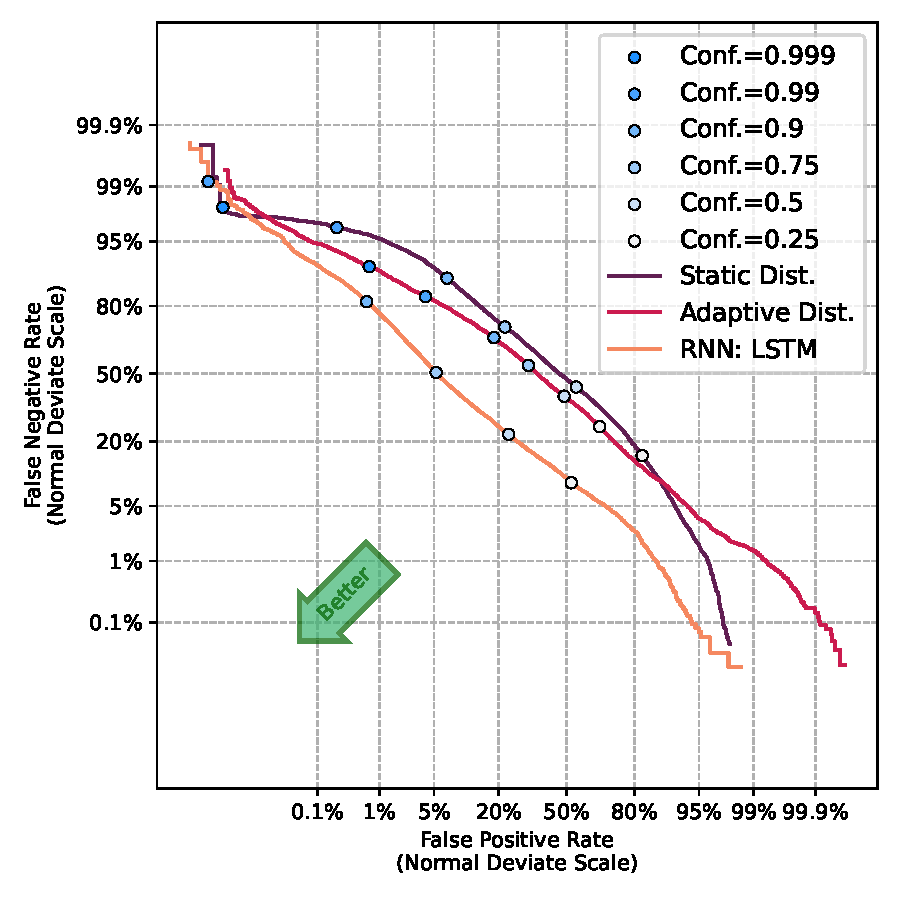
\includegraphics[width=.45\textwidth]    {figures/manuscript_det_curves_point_eval_gt_4xfwhm_v1.pdf}
    \caption{Point prediction performance for all three detectors over a range of thresholds.}
    \label{fig:point_prediction_performance}
\end{figure}

\subsection{Evaluation: Event Detections}
\label{subsec:evaluation_event_detections_results}

\begin{figure}
    \centering
    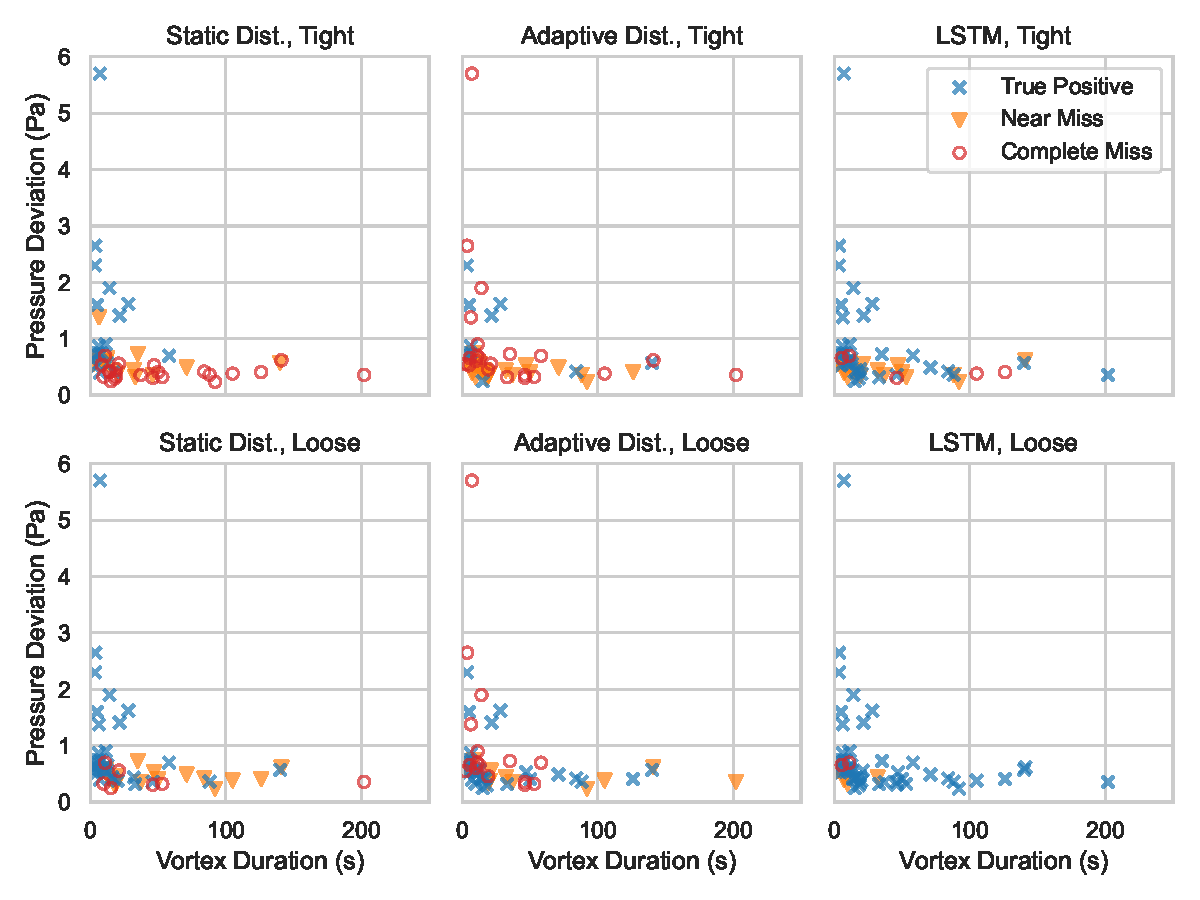
\includegraphics[width=.8\textwidth]    {figures/manuscript_system_performance_v1.pdf}
    \caption{Event detections for all three detectors using loose and tight filter thresholds.}
    \label{fig:system_performance}
\end{figure}

\begin{figure}
    \centering
    \includegraphics[width=0.45\textwidth]{example-image.pdf}
    \caption{Detection lead time between alert trigger and key science event.}
    \label{fig:detection_timing}
\end{figure}

\subsection{Science Analysis}
\todo{Brian and Chelle to draft}

\subsection{Resources Needed to Implement}
\subsubsection{Power and Data Volume to Collect Observations}
\subsubsection{Onboard Computing Power}
\subsubsection{Prior Knowledge about the Phenomenon}


\subsection{Informing Engineering Constraints}
